\documentclass[tikz,border=2pt]{standalone}
\usepackage[T1]{fontenc}
\usepackage{lmodern}
\usepackage{amsmath,amssymb}
\usetikzlibrary{arrows.meta,decorations.pathmorphing,decorations.pathreplacing,calc}
\definecolor{cblue}{HTML}{2b6cb0}
\definecolor{cdeep}{HTML}{1d4ed8}
\definecolor{cgold}{HTML}{b7791f}
\definecolor{cred}{HTML}{c0392b}
\definecolor{cgreen}{HTML}{1f8a5f}
\definecolor{tblue}{HTML}{e6eef8}
\definecolor{tgold}{HTML}{f8efdc}
\definecolor{tgray}{HTML}{efefef}
\definecolor{tgreen}{HTML}{e3f3eb}
\definecolor{cgray}{HTML}{8a8a8a}
\begin{document}
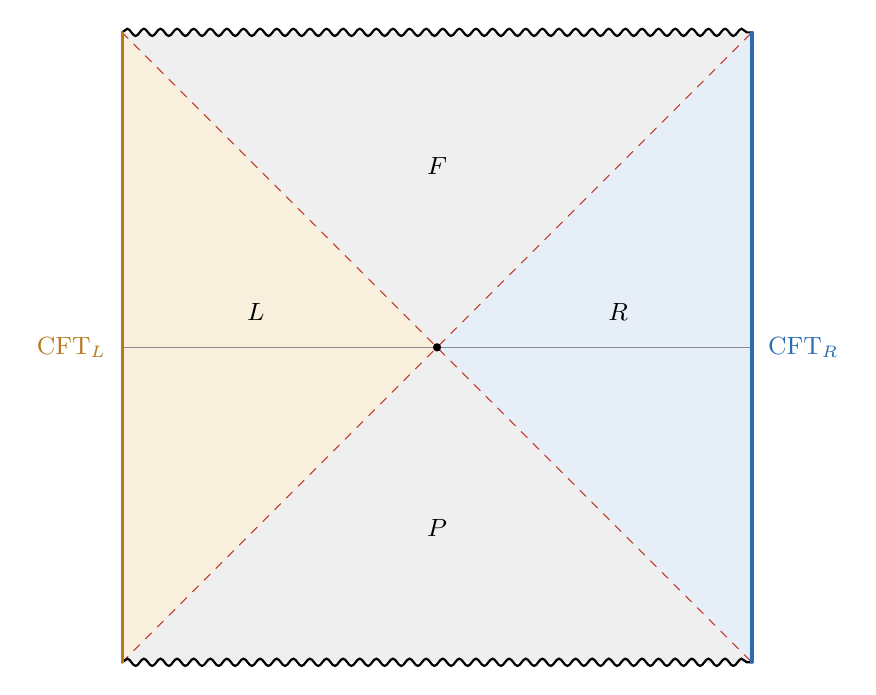
\begin{tikzpicture}[font=\small, line cap=round]
  \def\a{4}
  % regions
  \fill[tblue] (0,0) -- (\a,\a) -- (\a,-\a) -- cycle;       % R
  \fill[tgold] (0,0) -- (-\a,\a) -- (-\a,-\a) -- cycle;     % L
  \fill[tgray] (0,0) -- (-\a,\a) -- (\a,\a) -- cycle;       % F
  \fill[tgray] (0,0) -- (-\a,-\a) -- (\a,-\a) -- cycle;     % P
  % t = 0 slice through the Einstein--Rosen bridge
  \draw[cgray, thin] (-\a,0) -- (\a,0);
  % horizons
  \draw[cred, dashed, thin] (-\a,-\a) -- (\a,\a);
  \draw[cred, dashed, thin] (-\a,\a) -- (\a,-\a);
  % singularities
  \draw[decorate, decoration={snake, segment length=6pt, amplitude=1.3pt}, thick]
    (-\a,\a) -- (\a,\a);
  \draw[decorate, decoration={snake, segment length=6pt, amplitude=1.3pt}, thick]
    (-\a,-\a) -- (\a,-\a);
  % AdS boundaries
  \draw[cblue, line width=1.1pt] (\a,-\a) -- (\a,\a);
  \draw[cgold, line width=1.1pt] (-\a,-\a) -- (-\a,\a);
  % bifurcation point
  \fill (0,0) circle (1.5pt);
  % labels
  \node at ( 2.3, 0.45) {$R$};
  \node at (-2.3, 0.45) {$L$};
  \node at (0, 2.3) {$F$};
  \node at (0,-2.3) {$P$};
  \node[cblue, right] at (\a+0.08,0) {$\mathrm{CFT}_R$};
  \node[cgold, left]  at (-\a-0.08,0) {$\mathrm{CFT}_L$};
\end{tikzpicture}
\end{document}
